\section{Introduction}

\label{sec:Intro}

% Graph-- Uncertain Graph--Examples 
Graphs serve as powerful models to capture the complex relationships inherent among emerging applications, such as business to business (B2B) and social networks. Sometimes, the existence of the relationship between two entities is uncertain. 
For instance, in social networks, nodes represents individual users, while edges represent friendship or trust link among them derived by inference and prediction models built on interaction details~\cite{Lin_B2B,Adar_Managing_2007,Kempe_Maximizing_2003}, and edge probability may denote the accuracy of a link prediction, or the trust of one person on another. 
In these applications, the data can be modeled and shared as uncertain graphs whose edges carries a probability of existence. The probability represents the confidence that the relationship holds in reality. 

\begin{figure}[!htb]
  \vspace{-7pt}
    \subfigure[Social Trust Network]{\label{fig:socialNetwork}
      \begin{minipage}[l]{0.46\columnwidth}
        \centering
        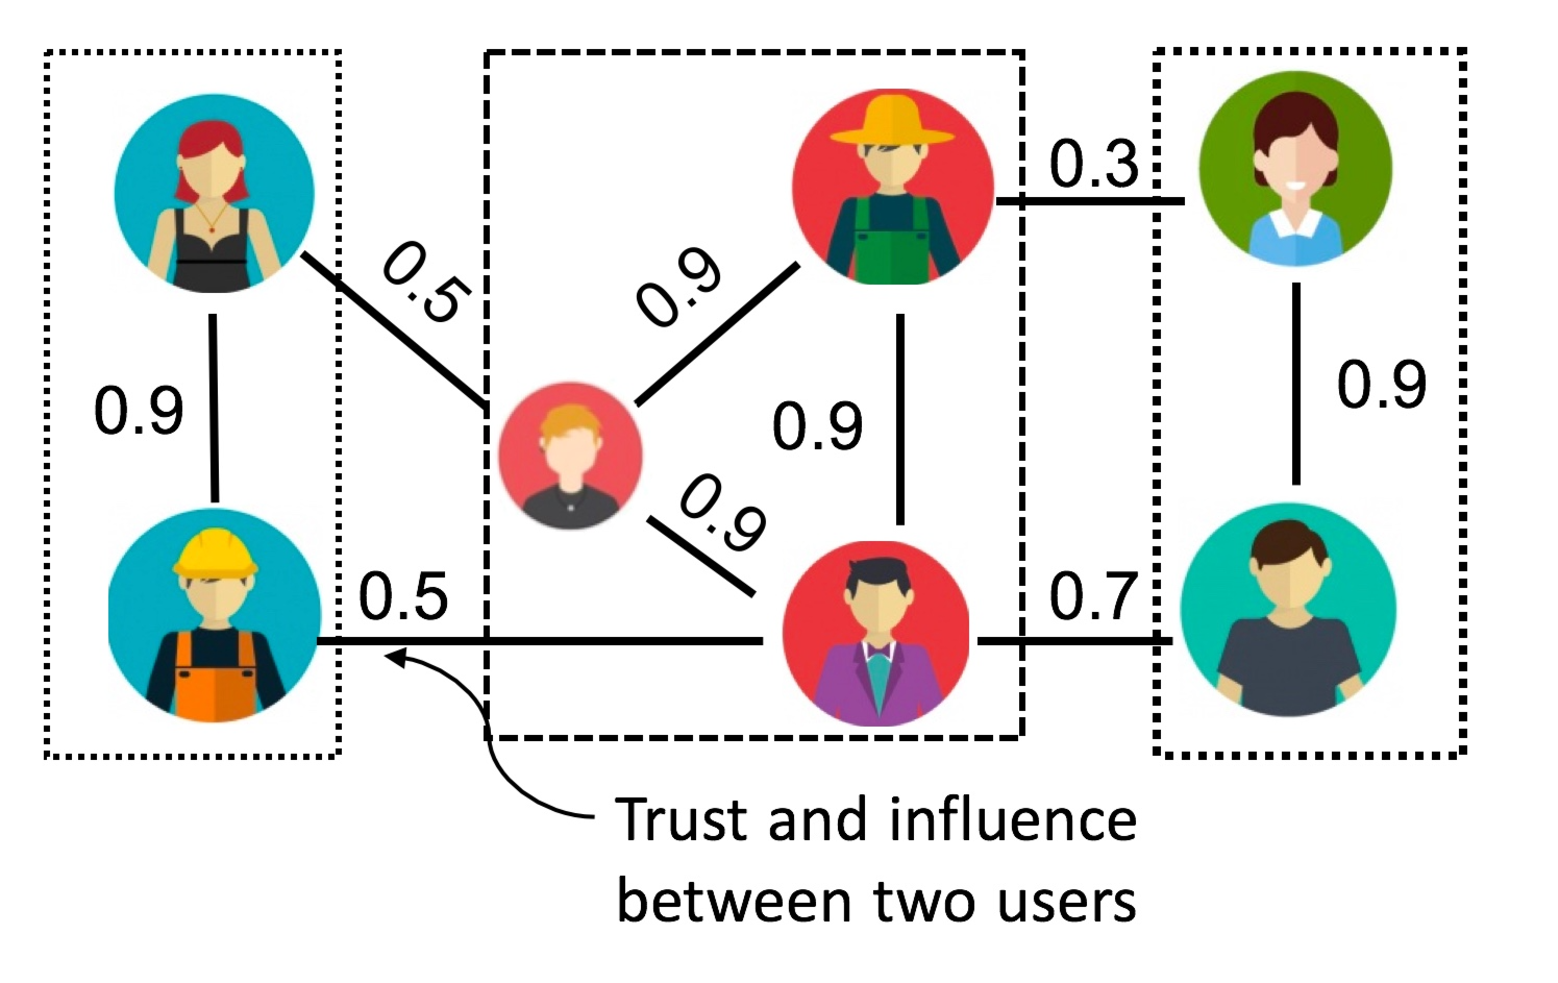
\includegraphics[height=2.7cm]{ill/SocialNetwork.pdf}
      \end{minipage}
      }
    \subfigure[B2B Network]{\label{fig:b2bNetwork}
      \begin{minipage}[l]{0.46\columnwidth}
        \centering
        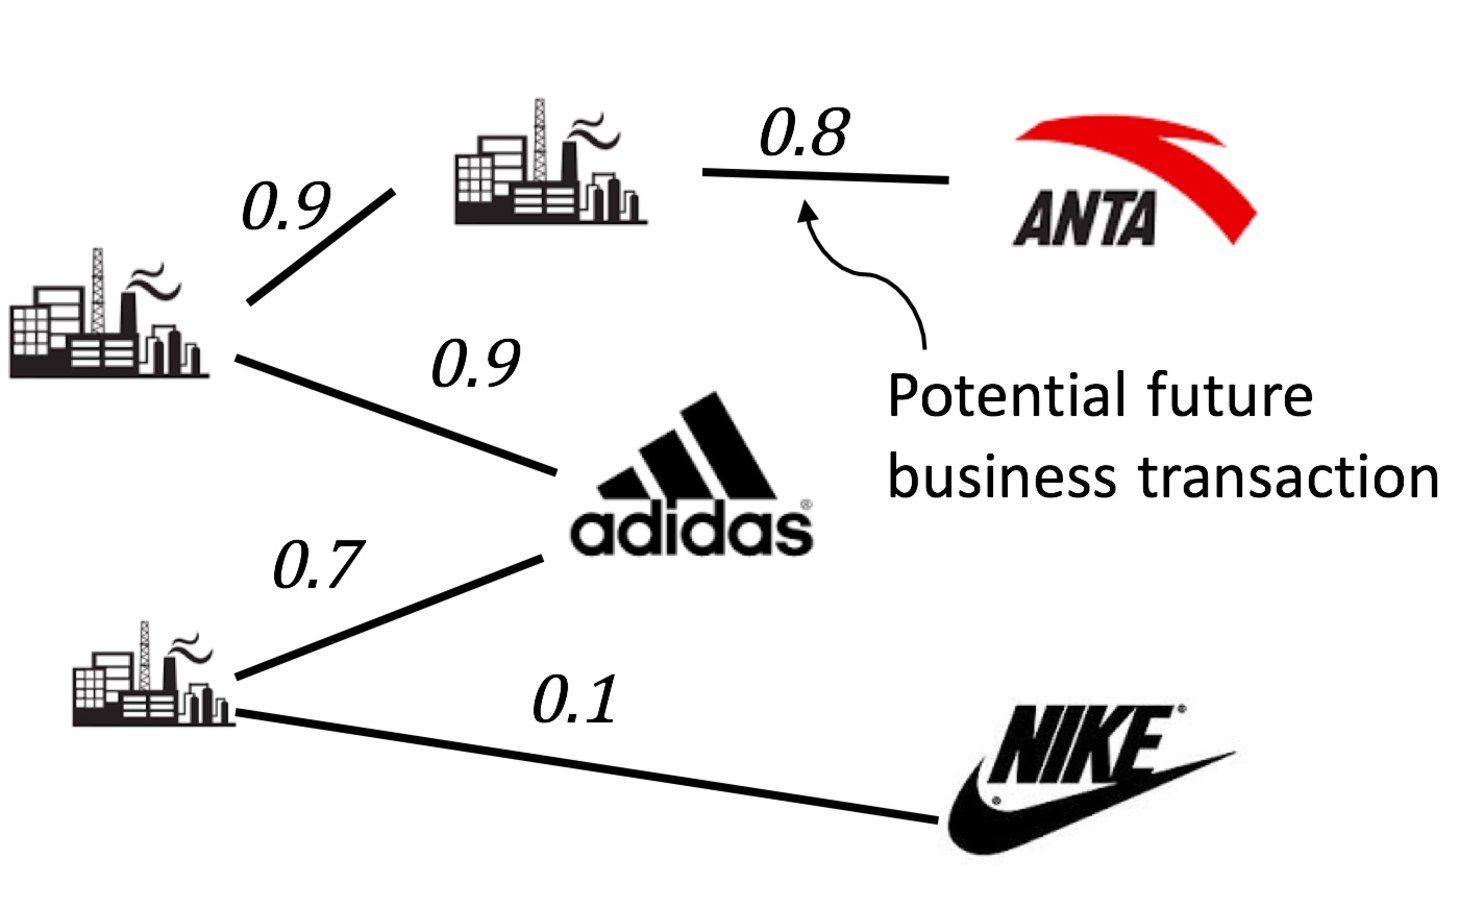
\includegraphics[height=2.7cm]{ill/B2BNetwork.pdf}
      \end{minipage}
      }
    \vspace{-7pt}
    \caption{Real-world uncertain graphs with privacy concerns.}
    \label{fig:motivation}
    \vspace{-7pt}
\end{figure} 

% Sharing--Privacy--Examples 
These uncertain graphs are invaluable for scientific research and commercial applications~\cite{Kempe_Maximizing_2003,Cho_Friendship_2011}. However, sharing these uncertain graphs would violate the privacy of users or entities profiled inside. For example, in social trust network, the trust and influence relationships among users---which may greatly impact users' behaviors, are usually probabilistic. Such uncertain graphs are useful in social interaction study, advertisement targeting and virtual marketing. While, users are unwilling to share such confidential information with the public or potential adversaries such as Cambridge Analysis. Similarly, in B2B networks, companies are unwilling to share their transaction patterns. Such tension is arising the question about sharing uncertain graphs without compromising privacy. 

% State-of-Art 
A number of privacy preserving graph sharing schemes have been studied in the deterministic scenario~\cite{Liu_Towards_2008,Ying_Randomizing_2008,Wang2011,Liu_Privacy_2009,Nguyen_Anonymizing_2015,Sala_Sharing_2011,Xiao_Differentially_2014,lee2011}, though many problems about sharing uncertain graphs still remain unexplored.

%weight casting fails 
An obvious approach is to convert uncertain graph sharing problem into the deterministic case by casting edge probabilities as edge weights. However, by disregarding the possible world semantic of uncertain graph, such an approach fails to reflect uncertain graph properties such as connectivity, dense subgraphs correctly, as witnessed by uncertain graph mining practices~\cite{Zhao_Detecting_2014,Hua_Probabilistic_2010}. Hence, a deterministic approach could produce very poor result.  

\textbf{Example.} Connectivity of deterministic subgraphs is generally measured by the concept of cut, which is defined as the sum of weights of intra edges. Generally, the bigger the cut, the harder to separate two subgraphs. In Figure~\ref{fig:socialNetwork}, the equal cut $C(SG_{1},SG_{2})=C(SG_{3},SG_{2})=1$ implies the identical connectivity of $SG_{1}$ and $SG_{3}$ w.r.t $SG_{2}$. However, with the possible world semantics, we know the probability to separate $SG_{1}$ and $SG_{2}$ is $(1-0.5)^{2}=0.25$, and that to separate $SG_{2}$ and $SG_{3}$ is $(1-0.3)(1-0.7)=0.21$. Hence, in fact, $SG_{2}$ is closer to $SG_{1}$ than to $SG_{3}$.

% Rep-OB 
In previous work~\cite{}, we ever present another option (Rep-Ob) which first extract a single representative instance from an uncertain graph as its approximation, then convert the problem into the deterministic case. However, this approach is shown to be problematic. The detachment of probabilities in the first step consequently deteriorates the overall data utility. 

In summary, either the ignorance or miscasting of edge probabilities makes these solutions inefficient for sanitizing uncertain graphs. In contrast, our work seeks a solution tailored towards uncertain graphs incorporating possible world semantics. We develop XX on the basis of syntactic private notation for sanitizing uncertain graphs. XX preserves as much stochastic nature of the original uncertain graph as possible, while injecting enough structural noise to guarantee a chosen level of privacy against re-identification attacks. To achieve this goal, we carefully addressed the following issues. 

$\bullet$~\textup{\emph{Stochastic Privacy Attacks.}}~~Edge uncertainty plays an indispensable
 role in uncertain graph model. It is impractical to discard them.  However, the additional release makes privacy protection far more difficult since it would empower the adversary and make the profiled entity more vulnerable to privacy attacks. Initially, we present and formulate potential kind of re-identification attacks and a extended version of syntactic privacy notation.

$\bullet$~\textup{\emph{Stochastic Utility Loss Metric.}}~~It is very challenging to maintain much stochastic nature when the uncertain graph is modified to pursue anonymity. The choice of utility loss metric does matter. Unfortunately, existing graph utility loss metrics such as graph edit distance~\cite{Liu_Towards_2008}, spectrum discrepancy~\cite{Ying_Randomizing_2008}, community reconstruction error~\cite{Wang2011} and shortest path discrepancy~\cite{Liu_Privacy_2009} are not good candidates because of the disregarding of edge probability. In this context, standard uncertain graph reliability 
discrepancy become a good criterion, because it evaluate the connectivity difference in the context of the entire graph and meanwhile utilizes the possible world model. 

$\bullet$~\textup{\emph{Intractable Search Space.}}~~Finding an sanitized uncertain graph with the desired level of privacy by as few graph contractions as possible is known to be NP-hard~\cite{Hartung_Theory_2015}. In the uncertain scenario, the edge modification is no longer a binary operation (addition/deletion), but there can be infinite probability values assigned to each edge. It becomes more computationally challenging.  

% change the sentence to be different to the original ones

% \hspace{-1em}


% \hspace{-1em}
% $\bullet$~\textup{\emph{Stochastic Utility Loss Metric.}}~~It is well-known that the choice of utility loss metric is critical for graph anonymization techniques. Some metrics such as graph edit distance~\cite{Liu_Towards_2008}, spectrum discrepancy~\cite{Ying_Randomizing_2008}, community reconstruction error~\cite{Wang2011} and shortest path discrepancy~\cite{Liu_Privacy_2009} are used in prior works. 
% While, they are heavily tailored for deterministic graphs and built on the top of deterministic graph concepts. Thus, they aren't right choices in the uncertain scenario. 
% We need a well-defined metric to accurately capture the structural deviation of uncertain graphs after anonymization.

% \hspace{-1em}
% $\bullet$~\textup{\emph{Intractable Search Space.}}~~Finding an anonymized graph with the desired level of privacy by as few graph contractions as possible is known to be NP-hard~\cite{Hartung_Theory_2015}. In this work, the edge operation is no longer a binary operation (addition/deletion), but there can be infinite probability values assigned to each edge. It becomes more computationally challenging.  








